% Set-up of the panel tests of Rajendran (2010), Secs. 5.5-5.7 (adapted from
% manuscript/figures/fig-panel.tex): (a) panel [0,2] x [-1,1], supports
% u_x(0,+-1) = 0 and u(0,0) = 0 (rp_model.m), output point A = (2,0);
% (b)-(d) the three load cases, equilibrated tractions on x = 0 and x = 2
% (rp_loads.m, rp_exact.m), arrows to scale within each case (shear tractions
% in (d) with their own scale); (e) super-element of 2 x 2 8-node elements:
% the four internal mid-side nodes are rotated counter-clockwise by theta
% about the centre node (schematic, theta = 135 deg).
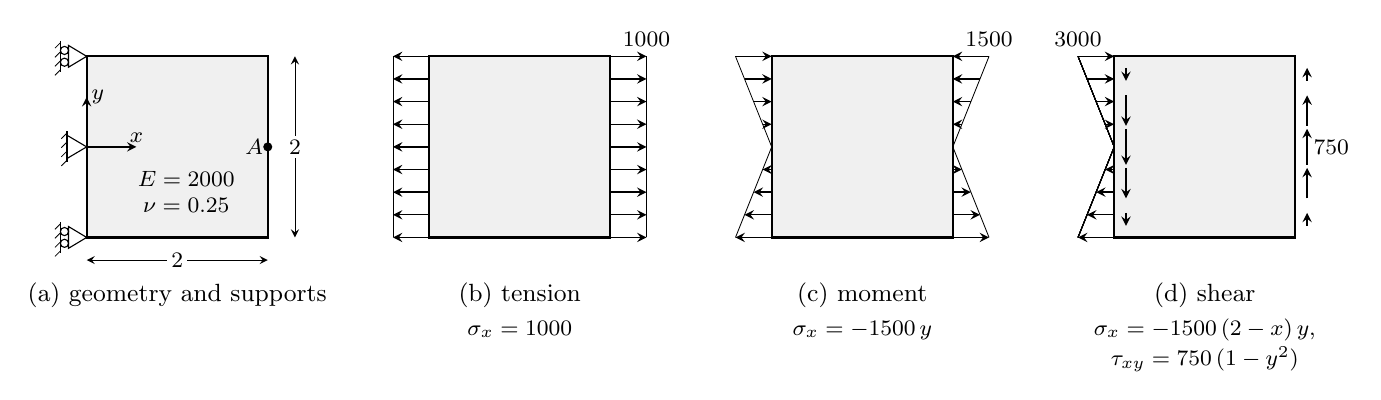
\begin{tikzpicture}[x=1.15cm, y=1.15cm,
    plabel/.style={anchor=north, font=\small, inner sep=0pt, align=center},
    slabel/.style={font=\footnotesize, inner sep=1.5pt},
    body/.style={draw=black, fill=gray!12, line width=0.8pt},
    trac/.style={-stealth, line width=0.5pt},
    roller/.pic={% apex at the node, restrains the displacement in the pic's x direction
      \draw[line width=0.4pt, fill=white] (0,0) -- (-0.2,0.12) -- (-0.2,-0.12) -- cycle;
      \draw[line width=0.4pt] (-0.245,0.065) circle (0.045) (-0.245,-0.065) circle (0.045);
      \draw[line width=0.6pt] (-0.29,0.17) -- (-0.29,-0.17);
      \foreach \s in {-0.15,-0.05,0.05,0.15} \draw[line width=0.3pt] (-0.29,\s) -- (-0.35,\s-0.06);},
    pin/.pic={% apex at the node, restrains both displacements
      \draw[line width=0.4pt, fill=white] (0,0) -- (-0.22,0.13) -- (-0.22,-0.13) -- cycle;
      \draw[line width=0.6pt] (-0.22,0.17) -- (-0.22,-0.17);
      \foreach \s in {-0.15,-0.05,0.05,0.15} \draw[line width=0.3pt] (-0.22,\s) -- (-0.28,\s-0.06);}]
% traction arrow at (#1,#2) on an edge with outward normal (#3,0), scaled
% traction (#4,#5): tail at the edge for tension, head at the edge for pressure
\def\panTrac#1#2#3#4#5{%
  \pgfmathsetmacro\pdn{(#4)*(#3)}%
  \pgfmathsetmacro\plen{veclen(#4,#5)}%
  \ifdim\plen pt>0.01pt
    \ifdim\pdn pt<0pt \draw[trac] ({#1-(#4)},{#2-(#5)}) -- (#1,#2);
    \else \draw[trac] (#1,#2) -- ++({#4},{#5});
    \fi
  \fi}
% (a) geometry and supports
\begin{scope}
  \draw[body] (0,-1) rectangle (2,1);
  \draw[-stealth, line width=0.5pt] (0,0) -- (0.55,0) node[slabel, above] {$x$};
  \draw[-stealth, line width=0.5pt] (0,0) -- (0,0.55) node[slabel, right] {$y$};
  \pic at (0,1) {roller};
  \pic at (0,-1) {roller};
  \pic at (0,0) {pin};
  \fill (2,0) circle (0.05) node[slabel, left] {$A$};
  \node[slabel, align=center] at (1.1,-0.5) {$E=2000$\\$\nu=0.25$};
  \draw[stealth-stealth, line width=0.3pt] (0,-1.25) -- node[slabel, fill=white] {$2$} (2,-1.25);
  \draw[stealth-stealth, line width=0.3pt] (2.3,-1) -- node[slabel, fill=white] {$2$} (2.3,1);
  \node[plabel] at (1,-1.5) {(a) geometry and supports};
\end{scope}
% (b) tension: sigma_x = 1000
\begin{scope}[xshift=4.35cm]
  \draw[body] (0,-1) rectangle (2,1);
  \foreach \y in {-1,-0.75,...,1} {
    \panTrac{2}{\y}{1}{0.4}{0}
    \panTrac{0}{\y}{-1}{-0.4}{0}}
  \draw[line width=0.3pt] (2.4,-1) -- (2.4,1) (-0.4,-1) -- (-0.4,1);
  \node[slabel, anchor=south, yshift=2pt] at (2.4,1) {$1000$};
  \node[plabel] at (1,-1.5) {(b) tension\\[1pt]\footnotesize $\sigma_x=1000$};
\end{scope}
% (c) pure bending: sigma_x = -1500 y (net moment 1000)
\begin{scope}[xshift=8.7cm]
  \draw[body] (0,-1) rectangle (2,1);
  \foreach \y in {-1,-0.75,...,1} {
    \panTrac{2}{\y}{1}{-0.4*\y}{0}
    \panTrac{0}{\y}{-1}{0.4*\y}{0}}
  \draw[line width=0.3pt] (2.4,-1) -- (2,0) -- (2.4,1) (-0.4,-1) -- (0,0) -- (-0.4,1);
  \node[slabel, anchor=south, yshift=2pt] at (2.4,1) {$1500$};
  \node[plabel] at (1,-1.5) {(c) moment\\[1pt]\footnotesize $\sigma_x=-1500\,y$};
\end{scope}
% (d) end shear: sigma_x = -1500 (2-x) y, tau_xy = 750 (1-y^2) (shear force 1000)
\begin{scope}[xshift=13.05cm]
  \draw[body] (0,-1) rectangle (2,1);
  % normal component on x = 0: t_x = 3000 y
  \foreach \y in {-1,-0.75,...,1}
    \panTrac{0}{\y}{-1}{0.4*\y}{0}
  \draw[line width=0.3pt] (-0.4,-1) -- (0,0) -- (-0.4,1);
  \node[slabel, anchor=south, yshift=2pt] at (-0.4,1) {$3000$};
  % shear component (own scale): t_y = 750 (1-y^2) on x = 2, -750 (1-y^2) on x = 0
  \foreach \y in {-0.8,-0.4,0,0.4,0.8} {
    \draw[trac] (2.13,{\y-0.2*(1-\y*\y)}) -- (2.13,{\y+0.2*(1-\y*\y)});
    \draw[trac] (0.13,{\y+0.2*(1-\y*\y)}) -- (0.13,{\y-0.2*(1-\y*\y)});}
  \node[slabel, right] at (2.15,0) {$750$};
  \node[plabel] at (1,-1.5) {(d) shear\\[1pt]\footnotesize $\sigma_x=-1500\,(2-x)\,y$,\\\footnotesize $\tau_{xy}=750\,(1-y^2)$};
\end{scope}
\end{tikzpicture}\par\bigskip
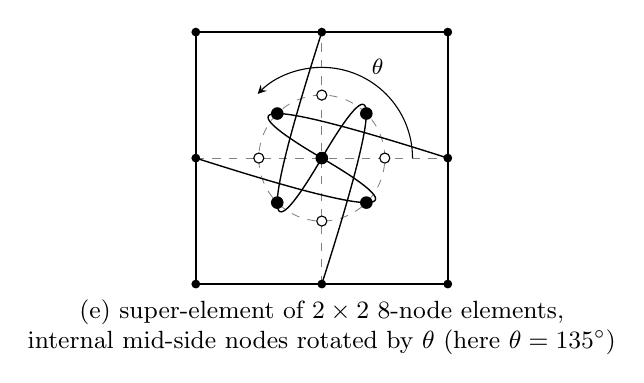
\begin{tikzpicture}[x=1.6cm, y=1.6cm,
    plabel/.style={anchor=north, font=\small, inner sep=0pt, align=center},
    slabel/.style={font=\footnotesize, inner sep=1.5pt}]
% (e) super-element of 2 x 2 elements: internal mid-side nodes rotated by theta
\def\th{135}
\draw[gray, dashed, line width=0.3pt] (-1,0) -- (1,0) (0,-1) -- (0,1);
\draw[gray, dashed, line width=0.3pt] (0,0) circle (0.5);
\foreach \k in {0,90,180,270}
  \draw[black, line width=0.5pt] plot[domain=-1:1, samples=41, variable=\s]
    ({0.5*cos(\k+\th)*(1-\s*\s) + cos(\k)*\s*(\s+1)/2},
     {0.5*sin(\k+\th)*(1-\s*\s) + sin(\k)*\s*(\s+1)/2});
\draw[line width=0.8pt] (-1,-1) rectangle (1,1);
\foreach \k in {0,90,180,270} {
  \draw[fill=white, line width=0.4pt] ({0.5*cos(\k)},{0.5*sin(\k)}) circle (0.04);
  \fill ({0.5*cos(\k+\th)},{0.5*sin(\k+\th)}) circle (0.05);
  \fill ({cos(\k)},{sin(\k)}) circle (0.035);}
\foreach \x/\y in {-1/-1,1/-1,1/1,-1/1} \fill (\x,\y) circle (0.035);
\fill (0,0) circle (0.05);
\draw[-stealth, line width=0.4pt] (0.72,0) arc[start angle=0, end angle=\th, radius=0.72];
\node[slabel, anchor=south west] at ({0.72*cos(60)},{0.72*sin(60)}) {$\theta$};
\node[plabel] at (0,-1.12) {(e) super-element of $2\times2$ 8-node elements,\\
  internal mid-side nodes rotated by $\theta$ (here $\theta=135^\circ$)};
\end{tikzpicture}
